% Created 2018-04-08 Sun 21:16
% Intended LaTeX compiler: pdflatex
\documentclass[11pt]{article}
\usepackage[utf8]{inputenc}
\usepackage[T1]{fontenc}
\usepackage{graphicx}
\usepackage{grffile}
\usepackage{longtable}
\usepackage{wrapfig}
\usepackage{rotating}
\usepackage[normalem]{ulem}
\usepackage{amsmath}
\usepackage{textcomp}
\usepackage{amssymb}
\usepackage{capt-of}
\usepackage{hyperref}
\usepackage{amssymb}
\usepackage{color}
\date{\today}
\title{}
\hypersetup{
 pdfauthor={},
 pdftitle={},
 pdfkeywords={},
 pdfsubject={},
 pdfcreator={Emacs 26.0.91 (Org mode 9.1.6)}, 
 pdflang={English}}
\begin{document}

\tableofcontents


\section{Spieltheorie}
\label{sec:org1e2df00}
In der Spieltheorie gibt es im Unterschied zur Entscheidungstheorie eine \textbf{Bimatrix} statt der Auszahlungsmatrix. In dieser sind die Einträge bereits \emph{Nutzengrößen}. Die Unsicherheit existiert nun nicht mehr im Hinblick auf Umweltzustände, sondern im Hinblick auf die Strategie eines weiteren Spielers. Da man nun die Auszahlungen für beide Spieler angeben muss, benötigt man zwei Matrizen \emph{oder} eine mit doppelten Einträgen, also eine "Bimatrix".
\begin{center}
\begin{tabular}{c|c|c|c}
S & s\(^{\text{1}}_{\text{2}}\) & s\(^{\text{2}}_{\text{2}}\) & s\(^{\text{3}}_{\text{2}}\)\\
\hline
s\(^{\text{1}}_{\text{1}}\) & (u\(_{\text{1}}\)(s\(^{\text{1}}_{\text{1,s}}\)\(^{\text{1}}_{\text{2}}\)), u\(_{\text{2}}\)(s\(^{\text{1}}_{\text{1}}\), s\(^{\text{1}}_{\text{2}}\))) & (u\(_{\text{1}}\)(s\(^{\text{1}}_{\text{1,s}}\)\(^{\text{2}}_{\text{2}}\)), u\(_{\text{2}}\)(s\(^{\text{1}}_{\text{1}}\), s\(^{\text{2}}_{\text{2}}\))) & (u\(_{\text{1}}\)(s\(^{\text{1}}_{\text{1,s}}\)\(^{\text{3}}_{\text{2}}\)), u\(_{\text{2}}\)(s\(^{\text{1}}_{\text{1}}\), s\(^{\text{3}}_{\text{2}}\)))\\
s\(^{\text{2}}_{\text{1}}\) & (u\(_{\text{1}}\)(s\(^{\text{2}}_{\text{1,s}}\)\(^{\text{1}}_{\text{2}}\)), u\(_{\text{2}}\)(s\(^{\text{2}}_{\text{1}}\), s\(^{\text{1}}_{\text{2}}\))) & (u\(_{\text{1}}\)(s\(^{\text{2}}_{\text{1,s}}\)\(^{\text{2}}_{\text{2}}\)), u\(_{\text{2}}\)(s\(^{\text{2}}_{\text{1}}\), s\(^{\text{2}}_{\text{2}}\))) & (u\(_{\text{1}}\)(s\(^{\text{2}}_{\text{1,s}}\)\(^{\text{3}}_{\text{2}}\)), u\(_{\text{2}}\)(s\(^{\text{2}}_{\text{1}}\), s\(^{\text{3}}_{\text{2}}\)))\\
s\(^{\text{3}}_{\text{1}}\) & (u\(_{\text{1}}\)(s\(^{\text{3}}_{\text{1,s}}\)\(^{\text{1}}_{\text{2}}\)), u\(_{\text{2}}\)(s\(^{\text{3}}_{\text{1}}\), s\(^{\text{1}}_{\text{2}}\))) & (u\(_{\text{1}}\)(s\(^{\text{3}}_{\text{1,s}}\)\(^{\text{2}}_{\text{2}}\)), u\(_{\text{2}}\)(s\(^{\text{3}}_{\text{1}}\), s\(^{\text{2}}_{\text{2}}\))) & (u\(_{\text{1}}\)(s\(^{\text{3}}_{\text{1,s}}\)\(^{\text{3}}_{\text{2}}\)), u\(_{\text{2}}\)(s\(^{\text{3}}_{\text{1}}\), s\(^{\text{3}}_{\text{2}}\)))\\
\end{tabular}
\end{center}
Die Nummer der Strategie ist nun im Gegensatz zu Kapitel 1 hochgestellt, unten steht die Nummer des Spielers.
\subsection{Beispiele}
\label{sec:orgec1cd5e}
\subsubsection{Hirschjagd}
\label{sec:org939a8a1}
\begin{center}
\begin{tabular}{c|c|c}
\textcolor{magenta}{Jäger 1}/\textcolor{blue}{Jäger 2} & \textcolor{blue}{Hirsch} & \textcolor{blue}{Hase}\\
\hline
\textcolor{magenta}{Hirsch} & (\textcolor{magenta}{5},\textcolor{blue}{5}) & (\textcolor{magenta}{0},\textcolor{blue}{4})\\
\textcolor{magenta}{Hase} & (\textcolor{magenta}{4},\textcolor{blue}{0}) & (\textcolor{magenta}{4},\textcolor{blue}{4})\\
\end{tabular}
\end{center}
\subsubsection{Kopf oder Zahl}
\label{sec:org094270b}
Jeder Spieler legt unbeobachtbar für den anderen Spieler eine Münze, stimmen die Bilder überein erhält Spieler 1 die Münzen, unterscheiden sie sich so erhält Spieler 2 die Münzen.
\begin{center}
\begin{tabular}{c|c|c}
\textcolor{magenta}{Spieler 1}/\textcolor{blue}{Spieler 2} & \textcolor{blue}{Kopf} & \textcolor{blue}{Zahl}\\
\hline
\textcolor{magenta}{Kopf} & (\textcolor{magenta}{1},\textcolor{blue}{-1}) & (\textcolor{magenta}{-1},\textcolor{blue}{1})\\
\textcolor{magenta}{Zahl} & (\textcolor{magenta}{-1},\textcolor{blue}{1}) & (\textcolor{magenta}{1},\textcolor{blue}{-1})\\
\end{tabular}
\end{center}
Ist ein Nullsummenspiel da \(E(\pi) = 0\)
\subsubsection{Kampf der Geschlechter}
\label{sec:orgff8a8ac}
\begin{center}
\begin{tabular}{c|c|c}
\textcolor{magenta}{Sie}/\textcolor{blue}{Er} & \textcolor{blue}{Theater} & \textcolor{blue}{Fußball}\\
\hline
\textcolor{magenta}{Theater} & (\textcolor{magenta}{4},\textcolor{blue}{3}) & (\textcolor{magenta}{2},\textcolor{blue}{2})\\
\textcolor{magenta}{Fußball} & (\textcolor{magenta}{1},\textcolor{blue}{1}) & (\textcolor{magenta}{3},\textcolor{blue}{4})\\
\end{tabular}
\end{center}
\subsubsection{Chicken/Hasenfuss-Spiel}
\label{sec:orga8f0d08}
\begin{center}
\begin{tabular}{c|c|c}
\textcolor{magenta}{Fahrer 1}/\textcolor{blue}{Fahrer 2} & \textcolor{blue}{geradeaus} & \textcolor{blue}{ausweichen}\\
\hline
\textcolor{magenta}{geradeaus} & (\textcolor{magenta}{0},\textcolor{blue}{0}) & (\textcolor{magenta}{4},\textcolor{blue}{2})\\
\textcolor{magenta}{ausweichen} & (\textcolor{magenta}{2},\textcolor{blue}{4}) & (\textcolor{magenta}{3},\textcolor{blue}{3})\\
\end{tabular}
\end{center}
\subsubsection{Gefangenendilemma}
\label{sec:org2642594}
\begin{center}
\begin{tabular}{c|c|c}
\textcolor{magenta}{Spieler 1}/\textcolor{blue}{Spieler 2} & \textcolor{blue}{schweigen} & \textcolor{blue}{gestehen}\\
\hline
\textcolor{magenta}{schweigen} & (\textcolor{magenta}{4},\textcolor{blue}{4}) & (\textcolor{magenta}{0},\textcolor{blue}{5})\\
\textcolor{magenta}{gestehen} & (\textcolor{magenta}{5},\textcolor{blue}{0}) & (\textcolor{magenta}{1},\textcolor{blue}{1})\\
\end{tabular}
\end{center}

Ein Spiel in strategischer Form ist ein Tripel: \(\Gamma = (I,(S_i)_{i \epsilon I} ,(u_i)_{i \epsilon I})\) \\
I = endliche, nichtleere Menge der Spieler zB: \{Unternehmen 1, Unternehmen 2\}\\
S = S\(_{\text{1}}\) x S\(_{\text{2}}\) x \ldots{} x S\(_{\text{i}}\) ist die Menge der Strategiekombinationen\\
S\(_{\text{i}}\) = die Strategiemenge jedes Spielers zB:

S\(_{\text{1}}\)=\{s\(^{\text{1}}_{\text{1}}\), s\(^{\text{2}}_{\text{1}}\)\}=\{Regenschirm, Sonnenschrim\}

S\(_{\text{2}}\)=\{s\(^{\text{1}}_{\text{2}}\), s\(^{\text{2}}_{\text{2}}\)\}=\{Sonnenschirm, Regenschirm\}

\(\rightarrow\) somit ist \(S = S_1 * S_2 = {(R,S), (R,R), (S,S), (S,R)}\) \\
u\(_{\text{i}}\) = die Auszahlungsfunktion eines jeden Spielers in Abhängigkeit von S zB für Spieler 1 von der Schirmproduktion:
\begin{center}
\begin{tabular}{ll}
\(u_1(R, S) = 10\) & \(u_1(R,R)=9\)\\
\(u_1(S, S) = 8\) & \(u_1(S,R)=11\)\\
\end{tabular}
\end{center}
und für Spieler 2:
\begin{center}
\begin{tabular}{ll}
\(u_2(R, S) = 5\) & \(u_2(R,R)=1\)\\
\(u_2(S, S) = 4\) & \(u_2(S,R)=2\)\\
\end{tabular}
\end{center}

\subsection{Beste Antworten}
\label{sec:org9b818d8}
Sei S\(_{\text{i}}\) eine Menge von Strategien aller anderen Spieler außer Spieler i. Dann liefert die Beste-Antwort-Korrespondenz B\(_{\text{i}}\) die Menge aller Strategien von Spieler i, die potenziell beste Antworten sein könnten. Eine beste Antwort auf eine Strategie ist
die Menge aller optimalen Reaktionen. Wenn es mehrere mögl. gegnerische Strategien gibt, dann gibt es dementsprechend auch mehrere mögliche beste Antworten.

\paragraph{Beispiel Hirschjagd:}
\(B_1(Hirsch) = Hirsch\) und \(B_1(Hase)=Hase\) das bedeutet die beste Antwort auf die gegnerische Strategie "Hirsch" ist für Spieler 1 Hirsch und auf Hase lautet die beste Antwort Hase.\\
\(B_2(Hirsch) = Hirsch\) und \(B_2(Hase)=Hase\) das bedeutet die beste Antwort auf die gegnerische Strategie "Hirsch" ist für Spieler 2 Hirsch und auf Hase lautet die beste Antwort Hase. \\
Alle Beste Antworten Spieler 1: \(B_1(\{Hirsch,Hase\})=\{Hirsch, Hase\}\) \\
Alle Beste Antworten Spieler 2: \(B_1(\{Hirsch,Hase\})=\{Hirsch, Hase\}\) 

\paragraph{Beispiel Chicken}
\begin{equation*}
\begin{aligned}
B_1(\{geradeaus, ausweichen\})= \{ausweichen, geradeaus\} \\
B_2(\{geradeaus, ausweichen\})= \{ausweichen, geradeaus\}
\end{aligned}
\end{equation*}

\paragraph{Beispiel Schirmproduktion}
\begin{equation*}
\begin{aligned}
B_1(\{S, R\})=\{R, S\} \\
B_2(\{S, R\})=\{S, S\} 
\end{aligned}
\end{equation*}

\subsubsection{Dominanz}
\label{sec:org2448d68}
Eine Strategie s\(_{\text{i}}\) dominiert(schwach) eine andere Strategie s'\(_{\text{i}}\) falls s\(_{\text{i}}\) für \textbf{alle gegnerischen} Strategien einen \textbf{mindestens gleichhohen} Nutzen wie s'\(_{\text{i}}\) liefert, formal: \\
\begin{equation*}
\begin{aligned}
u_i(s_i, s_{-i}) \geq u_i(s'_i, s_{-i})
\end{aligned}
\end{equation*}
für alle s\(_{\text{-i}}\) \(\epsilon\) S\(_{\text{-i}}\) also alle gegnerischen Strategien. Von strenger Dominanz spricht man wenn statt \(\ge\) ">" gilt.

\paragraph{Dominanz beim Gefangenendilemma}
\begin{center}
\begin{tabular}{c|c|c}
\textcolor{magenta}{Spieler 1}/\textcolor{blue}{Spieler 2} & \textcolor{blue}{schweigen} & \textcolor{blue}{gestehen}\\
\hline
\textcolor{magenta}{schweigen} & (\textcolor{magenta}{4},\textcolor{blue}{4}) & (\textcolor{magenta}{0},\textcolor{blue}{5})\\
\textcolor{magenta}{gestehen} & (\textcolor{magenta}{5},\textcolor{blue}{0}) & (\textcolor{magenta}{1},\textcolor{blue}{1})\\
\end{tabular}
\end{center}

Für Spieler 2 wird "schweigen" dominiert, denn 5 > 4 und 1 > 0. Spieler 1 antizipiert, dass Spieler 2 keine dominierte Strategie (also nicht "schweigen"), sondern "gestehen" spielen wird. Somit muss sich Spieler 1 dann nur noch zwischen 0 und 1 entscheiden da s\(^{\text{1}}_{\text{2}}\) wegfällt. Er wird gestehen wählen weil 1 > 0.

\subsubsection{Beste Antworten auf Wahrscheinlichkeitsverteilungen}
\label{sec:org10be366}
Angenommen die Gegenspieler haben gemischte Strategien. Dann liefert die Beste-Antwort-Korrespondenz B\(_{\text{i}}\) die Menge aller Beste-Antwort-Strategien. Es ändert sich eigentlich nichts, nur dass der Spieler i jetzt auf einen “unberechenbaren” Gegenspieler reagiert und die optimale Reaktion suchen muss.\\
Es werden also die besten Antworten auf Wahrscheinlichkeitsverteilungen gesucht:
\begin{center}
\begin{tabular}{c|c|c}
\textcolor{magenta}{Spieler 1}/\textcolor{blue}{Spieler 2} & \textcolor{blue}{Kopf}(\(\sigma_{\text{2}}\)) & \textcolor{blue}{Zahl}(1-\(\sigma_{\text{2}}\))\\
\hline
\textcolor{magenta}{Kopf}(\(\sigma_{\text{1}}\)) & (\textcolor{magenta}{1},\textcolor{blue}{-1}) & (\textcolor{magenta}{-1},\textcolor{blue}{1})\\
\textcolor{magenta}{Zahl}(1-\(\sigma_{\text{1}}\)) & (\textcolor{magenta}{-1},\textcolor{blue}{1}) & (\textcolor{magenta}{1},\textcolor{blue}{-1})\\
\end{tabular}
\end{center}
Erwarteter Nutzen Spieler 1:\\
\begin{equation*}
\begin{aligned}
u_i(\sigma_1,\sigma_2) = 1* \sigma_1* \sigma_2 + (-1) * \sigma_1 * (1- \sigma_2) + (-1)*(1- \sigma_1)* \sigma_2+1*(1-  \sigma_1)(1- \sigma_2)
\end{aligned}
\end{equation*}
Um herauszufinden wie Spieler 1 seinen Nutzen maximieren kann, muss diese Funktion partiel nach \(\sigma_{\text{1}}\) abgeleitet werden:\\
\begin{equation*}
\begin{aligned}
f'_{\sigma_1}=4 \sigma_2 - 2
\end{aligned}
\end{equation*}
wenn \(\sigma_2 = \frac{1}{2}\) ist, dann ist \(f'_{sigma_1}=0\) \(\rightarrow\) beste Antwort ist unbestimmt: \(\sigma_{\text{1}}\) \(\epsilon\) [0,1]\\
wenn \(\sigma_2 > \frac{1}{2}\) ist, dann ist \(f'_{sigma_1}>0\) \(\rightarrow\) beste Antwort ist \(\sigma_{\text{1}}\) = 100\% also ist BA die Wahl von Strategie s\(^{\text{1}}_{\text{1}}\)
wenn \(\sigma_2 < \frac{1}{2}\) ist, dann ist \(f'_{sigma_1}<0\) \(\rightarrow\) beste Antwort is \(\sigma_{\text{1}}\) = 0\% also ist BA die Wahl von Strategie s\(^{\text{2}}_{\text{1}}\)\\
\newpage
Beste Antwort von Spieler 1 auf Spieler \(\sigma_{\text{1}}\) in Abhängigkeit von \(\sigma_{\text{2}}\) sieht wie folgt aus:
\begin{center}
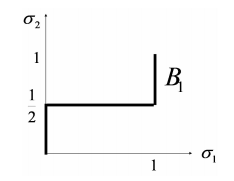
\includegraphics[width=100px]{./Kop_Zahl_BA.png}
\end{center}
\end{document}
